\documentclass[../main_zh.tex]{subfiles}

\graphicspath{{\subfix{../figures}}}

\begin{document}

\section{实验}\label{sec:experiment}

本节旨在通过全面的实验评估,验证我们提出的跨域 TNAS 框架 \OUR{} 的有效性。
我们在不同规模的搜索空间上进行了一系列实验,并对结果进行了深入分析。
此外,为了严格审查我们框架的各个组件和设计选择,我们设计了一系列研究进行更深层次的分析。
这些研究旨在阐明我们方法中每个关键元素的贡献,并为我们的方法论决策提供实证支持。

\subsection{搜索空间和数据集}

为了评估 \OUR{} 的有效性,我们设计了一套全面的实验,针对三个不同的 NAS 搜索空间:NAS-Bench-201、NAS-Bench-101 和 DARTS。
选择每一个都是为了例证不同层次的复杂性和架构约束,为我们的方法提供一个稳健的测试平台。

\textbf{NAS-Bench-201 空间.}\cite{DBLP:journals/pami/DongLMG22}\quad
该空间采用基于单元的设计,其中每个架构都被描绘成一个密集连接的有向无环图(DAG)。
它专门使用 OOE(操作在边上)方案,这意味着 DAG 中的每条边都代表一个特定的操作,
例如 \texttt{NONE}、\texttt{SKIP-CONNECT}、\texttt{CONV-1X1}、\texttt{CONV-3X3}
或 \texttt{AVG-POOL-3X3},应用于在节点之间流动的张量。
NAS-Bench-201 共包含 15,625 个独特的架构,每个架构有 4 个节点,为 NAS 算法的初步测试提供了一个紧凑而全面的框架。

\textbf{NAS-Bench-101 空间.}\cite{DBLP:conf/icml/YingKCR0H19}\quad
在复杂性方面更进一步,NAS-Bench-101 利用了基于单元的架构,其中 DAG 中的每个节点对应一个操作,符合 OON(操作在节点上)方案。
节点代表不同的操作,例如 \texttt{CONV-3X3}、\texttt{CONV-1X1} 和 \texttt{MAX-POOL-3X3},张量作为连接这些节点的边。
该搜索空间扩展到最多包含 7 个操作符且不超过 9 个连接的架构,从而产生 423,624 种独特的配置。
NAS-Bench-101 空间增加的表达能力和复杂性对 NAS 解决方案的适应性和可扩展性提出了挑战,使其成为复杂的领域。

\textbf{DARTS 空间.}\cite{DBLP:conf/iclr/LiuSY19}\quad
DARTS 代表了更高的复杂性,其架构以计算单元为特色,每个计算单元都建模为使用 OOE 方案的 DAG,类似于 NAS-Bench-201,但具有更高级的操作多样性。
在每个单元内,DAG 由 7 个节点的有序序列组成。
前两个节点被指定为输入张量,而最后一个节点用作输出张量。
DARTS 空间包括复杂的操作,包括 \texttt{MAX-POOL-3X3}、\texttt{AVG-POOL-3X3}、\texttt{SKIP-CONNECT}、\texttt{SEP-CONV-3X3}、\texttt{SEP-CONV-5X5}、\texttt{DIL-CONV-3X3} 和 \texttt{DIL-CONV-5X5}。
采用了两种不同的单元类型:保持空间分辨率的普通单元和对输入特征图进行下采样的缩减单元。
DARTS 空间包含了超过 \num{e18} 种普通和缩减单元的潜在组合,范围广阔。
该空间作为具有挑战性的领域,测试了框架处理复杂、大规模环境的能力以及在高度变化的架构设计中进行解决方案迁移的有效性。

\begin{table}
  \centering
  \caption{不同搜索空间上神经架构表示学习的超参数配置}\label{tab:train-settings}
  \renewcommand*{\arraystretch}{1.3}
  \newcommand*{\sizefn}{\tabularnote{用于训练的样本数,在括号中表示为占整个搜索空间的比例。其他大小相同。}}
  \newcommand*{\dartsfn}{\tabularnote{DARTS 搜索空间包含大量的神经架构,因此确定特定比例是不切实际的。}}
  \begin{NiceTabularX}{\linewidth}{@{}p{1.5cm}Xccc@}[notes,tabularnote={\textit{pt} = 预训练, \textit{ft} = 微调, \textit{repr} = 表示, \textit{ff} = 前馈, \textit{enc-lyr} = 编码器层, \textit{dec-lyr} = 解码器层.}]
    \toprule
                                             &                             & \bfseries NB201 & \bfseries NB101 & \bfseries DARTS          \\
    \midrule\midrule
    \Block{4-1}{\bfseries 训练设置} & \textit{pt-size}\\:\sizefn{} & 5,000~(0.5)     & 20,000~(0.5)    & 300,000~(--)\\:\dartsfn{} \\
                                             & \textit{ft-size}            & 1,000~(0.1)     & 4,000~(0.01)    & 1,500~(--)               \\
    \cmidrule{2-5}
                                             & \textit{pt-epoch}           & 200             & 200             & 200                      \\
                                             & \textit{ft-epoch}           & 200             & 200             & 200                      \\
    \midrule\midrule
    \Block{6-1}{\bfseries 模型设置}    & \textit{repr-dim}           & 64              & 64              & 128                      \\
                                             & \textit{model-dim}          & 128             & 128             & 512                      \\
                                             & \textit{ff-dim}             & 256             & 256             & 2,048                    \\
    \cmidrule{2-5}
                                             & \textit{n-enc-lyr}          & 4               & 4               & 4                        \\
                                             & \textit{n-dec-lyr}          & 4               & 4               & 4                        \\
                                             & \textit{n-head}             & 4               & 4               & 4                        \\
    \bottomrule
  \end{NiceTabularX}
\end{table}

\subsection{构建表示}

如第~\ref{sec:method-build-repre}节所述,首先为每个搜索空间构建表示。
表~\ref{tab:train-settings} 概述了用于训练与每个搜索空间相对应的表示学习器的超参数。
训练在单个 NVIDIA RTX2080Ti 上进行。
我们使用 AdamW 优化器,学习率设置为 \num{2e-5},权重衰减为 \num{1e-6}。
此外,还采用了\cite{DBLP:conf/nips/VaswaniSPUJGKP17} 中使用的调度器来调整学习率,预热期占总训练步数的 10%。
NAS-Bench-101 和 NAS-Bench-201 空间中的标签源自其各自的基准数据集,而 DARTS 空间缺少完整的基准数据集。因此,我们通过训练和收集必要的数据来为 DARTS 构建数据集。\footnote{这主要包括我们之前 NAS 过程中评估的神经架构的性能标签,以及来自 NAS-Bench-301 的训练集。}

\begin{table}[t]
  \centering
  \caption{神经架构表示学习方法的比较性能分析}\label{tab:repr-learn-metrics}
  \newcommand*{\trainfn}{\tabularnote{与其他方法不同,我们提出的方法保持了编码器和解码器的灵活性,从而能够将性能数据整合到表示学习中。然而,这导致了在重建准确性方面的一些折衷。}}
  \newcommand*{\dartsfn}{\tabularnote{结果基于我们在 DARTS 空间上收集的标签。}}
  \begin{NiceTabularX}{\linewidth}{p{6em}lXcccc@}[notes]
    \toprule
                                                                   &                                               &                                                   & \bfseries NB201 & \bfseries NB101 & \bfseries DARTS  \\
    \midrule\midrule
    \Block{5-1}{\bfseries 重建准确率 (\%)}             & \Block{5-1}{\bfseries\scriptsize\extuparrow} & \textit{arch2vec}~\cite{DBLP:conf/nips/YanZAZ020} & 99.99           & 98.84           & --               \\
                                                                   &                                               & SVGe~\cite{DBLP:conf/ijcnn/LukasikFZHK21}         & 99.99           & 99.57           & 99.63            \\
                                                                   &                                               & DGMG~\cite{DBLP:journals/corr/abs-1803-03324}     & 99.97           & 98.99           & 99.29            \\
    \cmidrule{3-6}
                                                                   &                                               & \OUR{} (预训练)                                     & 99.99           & 99.90           & 99.25            \\
                                                                   &                                               & \OUR{} (微调)                                     & 99.06           & 99.99           & 99.12            \\
    \midrule\midrule
    \Block{4-1}{\bfseries 预测 Kendall's \( \bm{\tau} \)-b} & \Block{4-1}{\bfseries\scriptsize\extuparrow} & NAO~\cite{DBLP:conf/nips/LuoTQCL18}               & 0.526           & 0.775           & --               \\
                                                                   &                                               & TNASP~\cite{DBLP:conf/nips/LuLTYL21}              & 0.724           & 0.820           & --               \\
                                                                   &                                               & ReNAS-6~\cite{DBLP:conf/cvpr/Xu00TJX021}          & --              & 0.816           & --               \\
    \cmidrule{3-6}
                                                                   &                                               & \OUR{}                                            & \textbf{0.827}  & \textbf{0.848}  & 0.811~\dartsfn{} \\
    \bottomrule
  \end{NiceTabularX}
\end{table}

表~\ref{tab:repr-learn-metrics} 描述了所提出的三元表示学习器的性能指标。第一部分涉及将表示重建为输入的准确性。高重建准确性表明 VAE 有效地封装了输入数据的基本特征。研究结果表明,所提出的方法在所有三个搜索空间中都实现了接近 100% 的重建准确性,表明构建了足够全面的神经架构表示。值得注意的是,VAE 的参数没有被冻结,从而允许将神经架构的性能信息集成到表示学习过程中。因此,可能会出现不可避免但可接受的重建准确性降低。

表~\ref{tab:repr-learn-metrics} 的下半部分展示了使用排序器进行微调的结果,重点关注排序器的性能预测与真实标签之间的排序相关性。
采用 \textit{Kendall's \( \tau \)-b 相关系数} (K-Tau) 来评估排序器指导迁移和搜索过程的能力。
所提出的预测器在 NAS-Bench-101 空间中实现了 0.809 的系数,在 NAS-Bench-201 空间中实现了 0.848 的系数,优于 NAO~\cite{DBLP:journals/corr/abs-1712-03351}、TNASP~\cite{E2EPPSun2023} 和 ReNAS~\cite{DBLP:conf/cvpr/Xu00TJX021} 中引入的方法。
此外,在 DARTS 空间中,我们获得了足够高的 K-Tau 分数 0.811,支持有效的架构迁移和搜索。
结果表明,通过表示预训练,我们的性能排序预测器实现了更高的准确性,并且与实际性能排名更紧密地对齐。

需要强调的是,这项工作的主要目标不是预测神经架构的性能。上述结果表明,所提出的方法有效地提取了神经架构的内在特征,并且能够对神经架构性能做出更准确的预测。表示学习为所提出的神经架构跨域迁移学习方法提供了基础理论。

\subsection{从简单域到复杂域的迁移}

\begin{figure}[t]
  \centering
  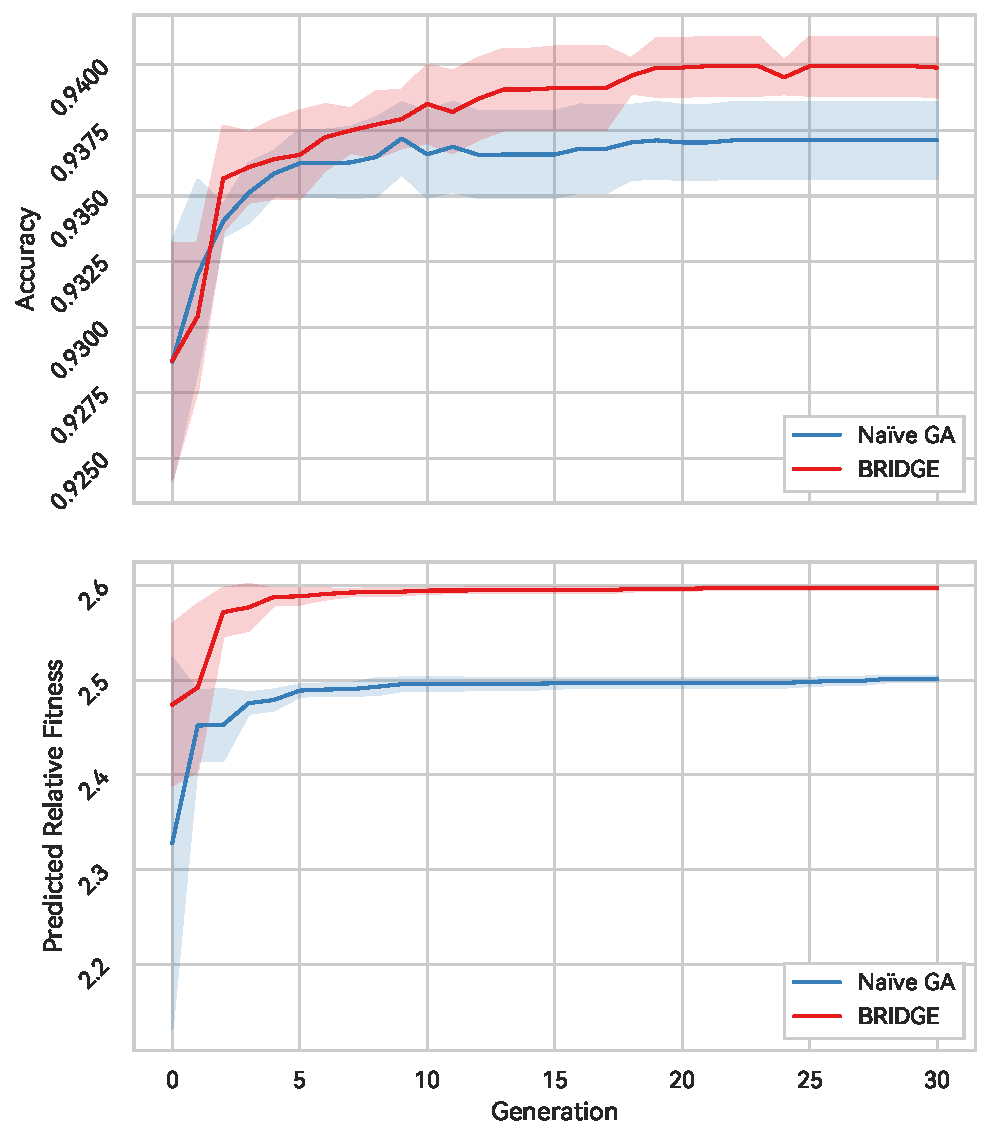
\includegraphics[width=\linewidth]{search-plot.pdf}
  \caption{
    % The fitness of the optimal solution for each population in the evolutionary NAS process with/without transfer.
    在使用和不使用 \OUR{} 的跨域 ESTO 机制的情况下,对 NAS-Bench-101 上的演化神经架构搜索性能进行的比较分析。
    \ \textit{上图:} 探索的架构在几代中的真实准确性。
    \ \textit{下图:} 来自排序器模块的预测相对适应度分数,该模块指导 NAS 过程作为评估策略。
  }\label{fig:search-process-plot}
\end{figure}

\begin{table*}[t]
  \centering
  \caption{NAS-Bench-101 空间上的神经架构搜索结果}\label{tab:transfer-result-101}
  \begin{NiceTabularX}{.8\linewidth}{X*{5}{c}}
    \toprule
    \bfseries 配置文件                         & \bfseries 最优准确率 (\%) & \bfseries 平均准确率 (\%) & \bfseries \#评估次数 & \bfseries 方法类型   \\
    \midrule\midrule
    ENAS~\cite{pham_efficient_2018}           & 92.54                       & 91.83\(\pm\)0.61          & --                  & 权重共享          \\
    FBNet~\cite{DBLP:conf/cvpr/WuDZWSWTVJK19} & 93.98                       & 92.29\(\pm\)1.84          & --                  & 基于梯度          \\
    CTNAS~\cite{DBLP:conf/cvpr/ChenGCLZWT21}  & 94.14                       & 93.93\(\pm\)0.42          & --                  & 预测器               \\
    ReNAS~\cite{DBLP:conf/cvpr/Xu00TJX021}    & 94.07                       & 93.95\(\pm\)1.25          & 423                 & 预测器               \\
    % NAO                                    &                             &                             &                     & representation learning \\
    SVGe~\cite{DBLP:conf/ijcnn/LukasikFZHK21} & 93.88                       & --                          & --                  & 表示学习 \\
    \midrule
    \RowStyle[nb-rows=4,color=BrickRed]{}
    PSO                                       & 93.77                       & 93.71\(\pm\)0.04          
    & --                  & \\
    PSO+\OUR{}                                & 93.96                       & 93.92\( \(\pm\)\)0.04          & --                  & \\
    MA & 94.07 & 93.93\(\pm\)0.36 & -- & \\
    MA+\OUR{} & 94.32 & 94.02\(\pm\)0.12 & -- & \\
    \midrule
    朴素 GA (基线)                  & 93.96                       & 93.71\(\pm\)1.74          & 500                 & 表示学习 \\
    \OUR{} (我们的)                             & \textbf{94.17}              & \textbf{93.99}\( \(\pm\)\)1.56 & 400                 & 表示学习 \\
    \bottomrule
  \end{NiceTabularX}
\end{table*}

我们通过从简单域到复杂域的迁移学习实验对所提出的方法进行了初步验证,具体来说,就是使用来自 NAS-Bench-201 空间的解决方案来增强在 NAS-Bench-101 空间中的搜索。
映射矩阵 \( \mathcal{M} \) 是通过分别从双方的训练集中采样 1,000 个解决方案来构建的。
我们选择了遗传算法 (GA)~\cite{HollandGA1992} 作为演化搜索求解器,这是一种在 NAS 中广泛使用的方法。
遵循~\cite{DBLP:conf/iconip/HouDFQ21} 中的设置,GA 求解器使用大小为 20 的种群,采用\textit{单点交叉}和\textit{多项式变异},概率均设置为 0.5,以及\textit{二元锦标赛选择}。

表~\ref{tab:transfer-result-101} 中呈现的结果将我们的方法与一个基线进行了比较,该基线由相同的 GA 求解器建立,但排除了所提出的跨域迁移方法(朴素 GA)。
我们的研究结果显著优于基线,在最优和平均准确率指标上均显示出显著的改进,值分别为 94.17% 和 93.99%。这证明了我们的迁移学习方法的有效性。
此外,我们的方法优于大多数现有的基于预测器的 NAS 方法,并且可以与这些方法集成以实现更稳健的结果。

为了进一步说明迁移学习对搜索过程的影响,图~\ref{fig:search-process-plot} 显示了种群最优解逐代变化的趋势。在早期阶段,迁移的解决方案创建了一个高质量且多样化的初始种群,从而能够从一开始就探索更优的解决方案区域。总之,我们提出的迁移学习方法有效地加速了神经架构搜索的过程,使其能够更早地收敛到更好的结果区域。


\subsection{向更具挑战性的领域迁移}

为了进一步评估我们迁移学习框架的稳健性,我们将评估扩展到更具挑战性的领域,特别关注 DARTS 空间。
如前所述,该空间代表了一个高度复杂的搜索环境。
与 NAS-Bench-101 和 NAS-Bench-201 相比,DARTS 空间提出了重大挑战,包括更广泛的可选操作、每个单元更多的操作,以及显著的两种不同单元类型的组合。
这些领域之间的巨大差异给迁移学习带来了相当大的挑战,使得本次评估尤为严格。

我们的实验设置涉及从 NAS-Bench-101 空间迁移知识,以告知和增强 DARTS 空间内的搜索。
表~\ref{tab:transfer-result-301} 总结了我们的方法与基线方法相比的性能。
值得注意的是,我们提出的 \OUR{} 实现了 97.33% 的准确率,显著优于基线方法。
这一结果证明了我们的方法能够有效地将知识迁移和适应到复杂领域。
为了提供额外的性能指标,我们利用 NAS-Bench-301 的性能预测器来评估我们发现的架构。
这一辅助措施为我们的方法在 DARTS 空间中的有效性提供了进一步的验证。

这些结果强调了我们的方法对各种复杂架构设计的适应性。
这种适应性对于应对大规模搜索空间带来的挑战至关重要,从而验证了我们框架在实际场景中的实用性。
此外,在高度不相似的领域之间成功迁移表明,我们的表示学习方法有效地提取了神经架构的潜在语义信息。
这种连接不同领域的能力可以显著推动自动机器学习领域的发展,从而在广泛的任务和领域中实现更高效、更有效的架构发现。

% The robustness of our transfer learning framework is further evaluated by transferring knowledge to more challenging domains. Specifically, we explore the DARTS space, which represents a highly complex search space as menthoned above.
% Compared to NAS-Bench-101 and NAS-Bench-201, the DARTS space encompasses more optional operations, a greater number of operations, and, notably, a combination of two types of cells.
% The significant differences between domains present challenges for transfer learning.
% This section aims to illustrate the efficacy of our method in handling such a vast and intricate architecture space.

% For these settings, we utilized the solutions from the NAS-Bench-101 space to inform and enhance the search within the DARTS space. As summarized in Table~
ef{tab:transfer-result-301}, demonstrate the performance of our approach compared to baseline methods. Our framework significantly outperforms baseline approach with the accuracy of 97.33%, showcasing its ability to transfer and adapt knowledge to complex domains effectively. In addition, we also used the performance predictor provided by NAS-Bench-301 to predict our architecture as an auxiliary metric.

% The result underscores the adaptability of our method to varied and complex architectural designs. This adaptability is key to addressing the challenges posed by large-scale search spaces, validating the practical applicability of our framework in real-world scenarios. Furthermore, the transfer across domains with high dissimilarity demonstrates that our representation learning extracts the underlying semantic information of the neural architecture.

\begin{table}
  \centering
  \caption{DARTS 空间上的神经架构搜索结果}\label{tab:transfer-result-301}
  % \begin{NiceTabularX}{\linewidth}{X*{3}{>{\centering\arraybackslash}X}}
  \begin{NiceTabularX}{.95\linewidth}{X*{3}{>{\centering\arraybackslash}p{5em}}}
    \toprule
    \bfseries 配置文件        & \Block{1-1}{\bfseries 最优准确率 (\%)} & \Block{1-1}{\bfseries NB301 预测} & \bfseries \#查询次数 \\
    \midrule\midrule
    朴素 GA (基线) & 96.62                                    & 94.85                                   & 600                 \\
    \OUR{} (我们的)            & \bfseries 97.33                          & \bfseries 94.93                         & 600                 \\
    \bottomrule
  \end{NiceTabularX}
\end{table}

\subsection{更深入的分析}

\subsubsection{超参数敏感性分析}\label{sec:hyperparam-analysis}

\begin{figure}
  \centering
  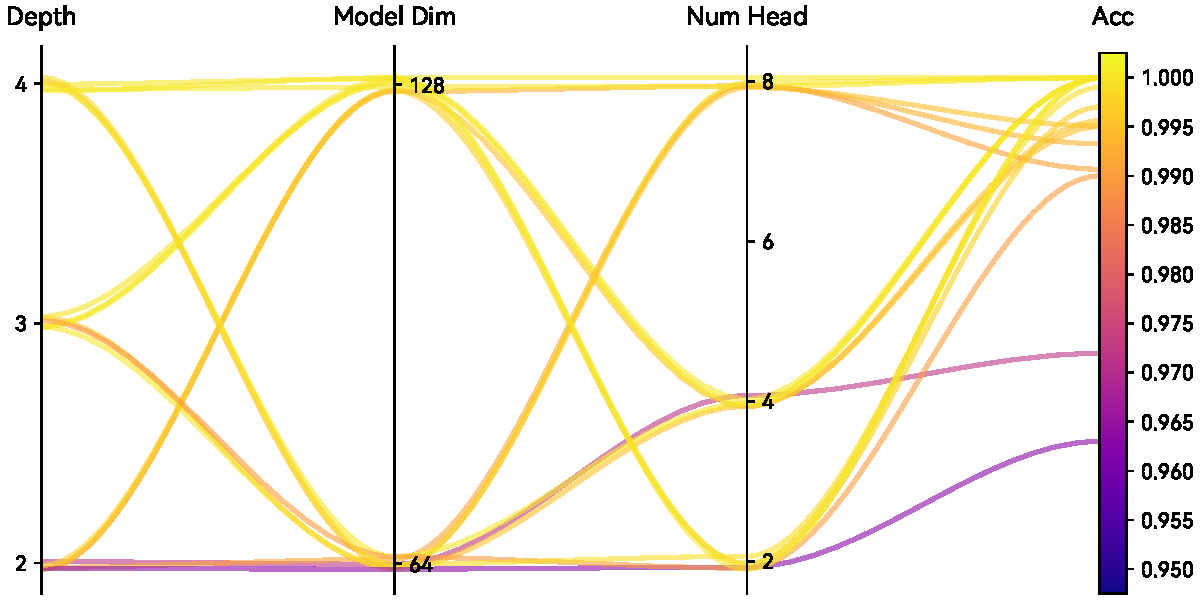
\includegraphics[width=.95\linewidth]{hpsa.pdf}
  \DiffBegin
  \caption{
    并行坐标图显示了在不同超参数设置下,所提出的表示学习器在 NAS-Bench-101 上的准确性。
    每条线对应于网络深度、模型维度和注意力头数的唯一组合,而色阶表示最终的准确性(较暗的线表示较低的准确性,较亮的线表示较高的准确性)。
  }\label{fig:hyperparam-sensitivity}
  \DiffEnd
\end{figure}

\subsubsection{潜在表示空间观察}\label{sec:repre-space-analysis}

为了在整个训练过程中更直观地表示潜在表示空间内不断变化的分布,我们采用\textit{多维缩放} (MDS)~\cite{DOUGLASCARROLL1998179} 进行可视化。
此外,我们根据采样点的真实标签对其进行颜色编码,以方便解释。
如图~\ref{fig:nb101-mds} 所示,在表示学习过程的各个阶段,具有相似性能指标的神经架构在潜在表示空间内表现出空间邻近性。
这种聚合在训练过程中表现出逐步、阶梯式增加的连贯性。

观察到的聚类行为与 VAE 的固有属性一致。在预训练阶段,VAE 自然地倾向于将相似的神经架构放置在潜在空间中的邻近位置。此外,具有结构相似性的架构有更高的概率表现出可比的性能特征。这种内在的组织为后续性能排序器的训练提供了坚实的基础。
在微调阶段,引入源自真实标签的监督信号进一步增强了模型捕获有助于性能差异的特征的能力。这种改进反映在潜在空间分布中,其中具有相似性能指标的神经架构的表示显示出显著的聚合。
% In order to more intuitively represent the changes in the distribution of the latent representation space throughout the training process, we visualize the latent representation space through Multi-Dimensional Scaling (MDS).
% In addition, we colored the sampled points according to ground-truth labels.
% As shown in the Fig.~
ef{fig:nb101-mds}, neural architectures with similar performance are closer to each other in the latent representation space at various stages of representation learning.
% This aggregation admits a stepwise increase.

% Based on the nature of VAE, similar neural architectures will be close together in the latent space during the pre-training process; what's more, similar architectures have a higher probability of having similar performance.
% This provides a good basis for the subsequent training of the performance ranker.
% And in the fine-tuning phase, after the engagement of supervisory signals from ground-truth labels, our representation learning model captures well the features that lead to performance differences, which is reflected in the distribution of the latent space, where similarly performing neural architecture representations exhibit remarkable aggregation.

\begin{figure}
  \centering
  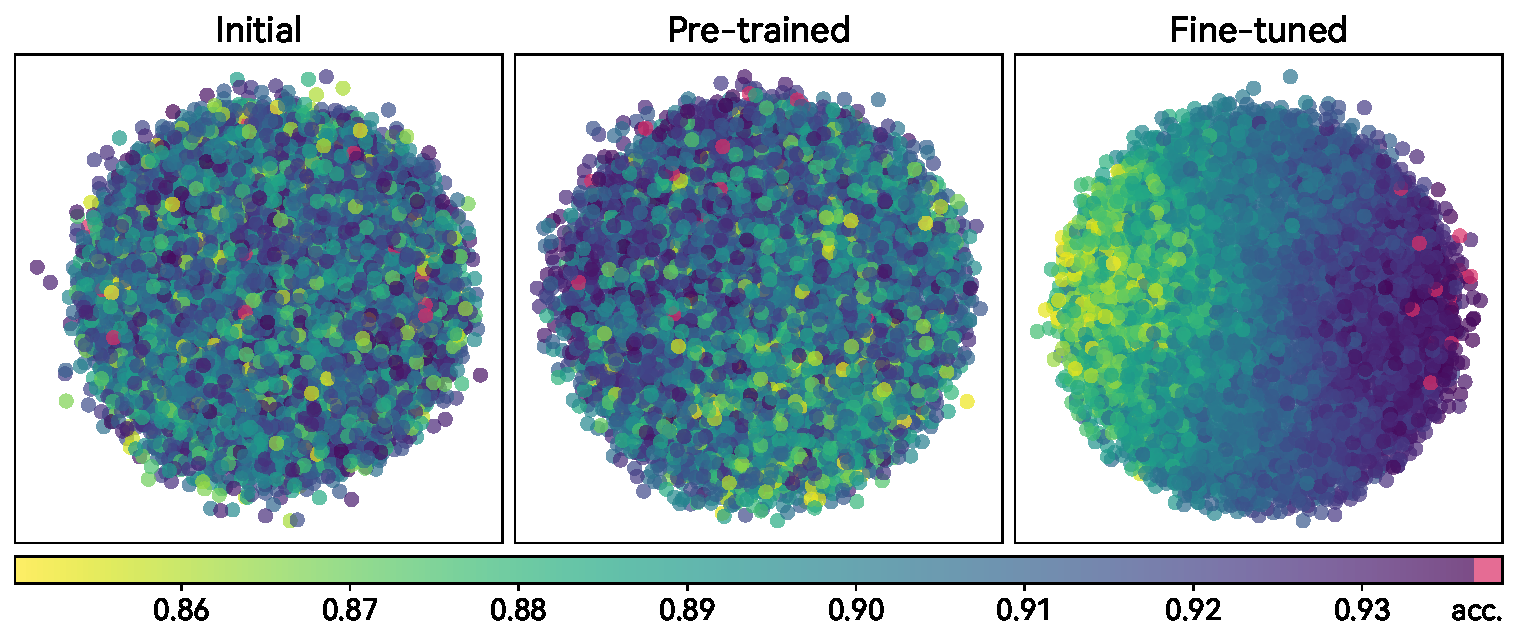
\includegraphics[width=.95\linewidth]{nb101-mds.pdf}
  \caption{
    % Visualization of the representation space on the NAS-Bench-101 search space.
    在不同训练阶段(初始(左)、预训练后(中)和微调后(右))学习到的 NAS-Bench-101 架构表示空间的可视化。
    颜色表示架构性能(准确性),暖色代表更高的准确性。
  }\label{fig:nb101-mds}
\end{figure}

\subsubsection{所用训练数据量的影响}

\begin{table}
  \centering
  \caption{在 NAS-Bench-101 上预训练阶段的神经架构表示学习性能,在不同数据集大小下进行评估}\label{tab:ablation-pretrin-data-size}
  \newcommand*{\ablationfn}{\tabularnote{为了消除实验中预测器的干扰,我们在不同数据集大小之间使用统一的性能预测器。}}
  \begin{NiceTabularX}{\linewidth}{p{12em}*{5}{>{\centering\arraybackslash}X}}
    \toprule
    \bfseries 未标记数据 & \bfseries 1\% & \bfseries 5\% & \bfseries 10\% & \bfseries 30\% & \bfseries 50\% \\
    \midrule\midrule
    \textbf{VAE 准确率} (\%)   & 78.82         & 89.46         & 99.91          & 99.56          & 99.97          \\
    \textbf{成本} (GPU 天) & 0.08          & 0.08          & 0.08           & 0.11           & 0.15           \\
    \bottomrule
  \end{NiceTabularX}
\end{table}

\begin{table}
  \centering
  \caption{在 NAS-Bench-101 上微调阶段的神经架构表示学习性能,在不同数据集大小下进行评估}\label{tab:ablation-finetune-data-size}
  \newcommand*{\ablationfn}{\tabularnote{为了消除实验中预测器的干扰,我们在不同数据集大小之间使用统一的性能预测器。}}
  \begin{NiceTabularX}{\linewidth}{p{12em}*{3}{>{\centering\arraybackslash}X}}
    \toprule
    \bfseries 标记数据              & \bfseries 0.1\% & \bfseries 1\% & \bfseries 5\% \\
    \midrule\midrule
    \bfseries Kendall's \(\bm{\tau}\)-b & 0.738           & 0.848         & 0.865         \\
    \bfseries 成本 (GPU 天)           & 0.01            & 0.02          & 0.02          \\
    \textbf{最优结果}             &                 &               &               \\
    \quad --- 作为源(\%)            & 96.56           & 97.33         & 97.36         \\
    \quad --- 作为目标(\%)            & 93.68           & 94.17         & 94.24         \\
    \bottomrule
  \end{NiceTabularX}
\end{table}
表示学习模型是我们提出的迁移框架的基本组成部分,对知识迁移的有效性起着重要作用,因此也决定了性能结果。
我们的表示学习模型训练方法包括两个阶段:无监督预训练和有监督微调。
如第~\ref{sec:repre-space-analysis}节所述,微调阶段对于对齐跨域表示空间尤为重要。鉴于标记数据对模型微调的关键影响,我们对不同数据比例对 NAS-Bench-101 上神经架构表示学习的影响进行了调查。

表~\ref{tab:ablation-pretrin-data-size} 展示了在一系列数据集大小下神经架构表示学习的关键性能指标。
在微调期间,VAE 在不同数据集大小下表现出稳健的性能,实现了至少 99.90% 的准确率,表明即使数据有限,它也能始终如一地捕获神经架构的底层结构。
这表明无监督学习有效地建模了架构特征,尽管数据量有所不同。
然而,预测器组件的性能对训练数据量表现出更大的敏感性。
随着数据集大小的增加,K-Tau 得到改善,在数据集的 5% 处达到最大值 0.862,反映出更大数据集具有更强的预测性能。

这种敏感性不仅体现在预测准确性上,还影响了学习到的表示空间的分布特征。
我们的研究结果表明,更大的标记数据集有助于形成一个结构更清晰、组织更良好的表示空间,从而促进学习更精确的域间映射函数。这种改进的结构和域间映射准确性的提高直接增强了目标任务上的搜索性能。
例如,使用总数据集的 5%,我们作为源域实现了 97.36% 的准确率,作为目标域实现了 94.24% 的准确率,说明了更大数据集对跨域可迁移性的好处。

总之,虽然 VAE 对有限数据表现出弹性,但性能预测器和迁移学习阶段从更大数据集中获益匪浅。这凸显了在迁移学习场景中数据采集和整理的重要性,尤其是在旨在优化标记数据有限的目标域中的性能时。



% Crucially, our findings indicate that larger labeled datasets contribute to the construction of a more well-structured representation space.
% This enhanced structure facilitates the learning of more accurate mapping functions between domains.
% The improved quality of the representation and the increased accuracy of the inter-domain mapping subsequently translate to enhanced search performance on the target task.
% Based on 5% of total dataset, we get accuracies of 97.36% (as source domain) and 94.24% (as target domain), respectively.
% These results highlight the nuanced relationship between data availability and the efficacy of cross-domain TNAS\@.
% While the pre-training phase demonstrates resilience to data limitations, the supervised fine-tuning and subsequent transfer learning processes benefit significantly from larger datasets.
% This underscores the importance of data acquisition and curation in transfer learning scenarios, particularly when aiming to optimize performance in target domains with limited labeled data.

% The representation model, central to the proposed transfer framework, is pivotal to the final outcome. In training the representation learning model, we employ an unsupervised pre-training phase followed by a supervised fine-tuning approach. Data is a critical factor influencing model training. We investigate the impact of varying data ratios on neural architecture representation learning.

% Table~
ef{tab:ablation-data-size} presents key indicators of neural architecture representation learning across varying dataset sizes. Our analysis reveals that the pre-training phase renders the VAE robust to dataset size variations, maintaining consistent reconstruction accuracy across different data volumes. In contrast, the predictor exhibits higher sensitivity to the training dataset size. This sensitivity not only affects prediction accuracy but also influences the distribution characteristics of the learned representation space. 

% Importantly, our results indicate that larger labeled datasets contribute to the construction of a more well-structured representation space. This enhanced structure facilitates the learning of more accurate mapping functions between domains. The improved representation quality and mapping accuracy subsequently translate to enhanced search performance on the target task, underscoring the importance of sufficient data in transfer learning scenarios.


% As shown in Table~
ef{tab:ablation-data-size}, we selected key indicators of neural architecture representation learning. Thanks to the pre-training phase, the dataset size does not significantly affect the reconstruction accuracy of the VAE. However, the predictor demonstrates higher sensitivity to the training dataset size, which also influences the distribution of the representation space. The results indicate that a larger number of labeled data points contributes to the construction of a well-structured representation space, facilitates the learning of more accurate mapping functions, and ultimately enhances search performance on the target task. The dataset size required for training the predictor is sufficient to support the transfer learning of the neural architecture.

\end{document}